% the following line is added to eliminate warnings about fonts on Mac
\PassOptionsToPackage{quiet}{fontspec} 

% use ctexarticle and include own package hw-cn.sty
\documentclass[]{ctexart}
\usepackage{hw-cn}

\usepackage{inputenc}
\usepackage{amsfonts,amsmath,amscd,amssymb,amsthm}
\usepackage{latexsym,bm}
\usepackage{cite}
\usepackage{mathtools,mathdots,graphicx,array}
\usepackage{fancyhdr}
\usepackage{lastpage}
\usepackage{color}
\usepackage{enumitem}
\usepackage{diagbox}
\usepackage{xcolor,tcolorbox,tikz,tkz-tab,mdframed,tikz-cd}
\usepackage{framed}
\usepackage{verbatim}
\usepackage{extarrows}
\usepackage{fontspec}
\usepackage{subfigure}
\usepackage{float} % use H command to fix position of figures
\usepackage{graphicx}
\usepackage{listings}
\usepackage{hyperref}
\usepackage{makecell}
\usepackage{bbding}


\newcommand\course{智能感知认知实践}
\newcommand\labnumber{任务}
\newcommand\name{孙一林}
\newcommand\stuID{520030910361}

\pagestyle{fancyplain}
\headheight 25pt
\lhead{\name \\ \stuID}
\chead{\textbf{\Large 语言模型\labnumber}}
\rhead{\course \\ \today}

\begin{document}

\section{提交文件简要说明}
本次实验使用实验室服务器进行训练,代码在超算中提供的代码框架基础上进行了更改。提交文件夹中,\texttt{checkpoint}目录下是实验运行结果,
包括各种模型在不同超参数下的实验日志,不同模型以不同的文件夹区分,而模型超参数则保存在\texttt{.txt}文件名中。
\texttt{tensorboard}文件夹下则保存了不同模型、参数下\texttt{SummaryWriter}的运行日志,即\texttt{events.out.tfevents.}前缀文件。
\section{各语言模型结构的理解}

\subsection{RNN}
传统RNN\ref{rnn}的引入是为了解决时间序列中相邻的观察之间具有依赖关系的问题。时间序列数据和普通的数据有着一定的差异,表现为当前的数据依赖于之前的数据,或者说,观察之间不是相互独立的。
然而,传统的神经网络却将每个观察视为独立的,而RNN通过包含数据点之间的依赖关系将记忆的概念引入神经网络,这样的一种假设和设计就使得RNN能够在具有依赖关系的数据集上表现显著优于传统神经网络。
通过所谓的反馈回路,一个RNN单元的输出也被同一单元用作输入。因此可以认为,每个RNN都有两个输入,即来自过去和现在的信息。
通过使用过去的信息,RNN在某种程度上实现了“短期记忆”,RNN的每个神经元都能同时接收当前时间步的输入、前一时间步的隐藏状态和偏置组合,然后仍通过激活函数,得到当前时间的状态。
RNN的这种实现不但能够通过短期记忆来处理顺序数据并识别历史数据中的模式,还能够处理不同长度的输入。

和传统神经网络一样,RNN也存在梯度消失的问题。由于在反向传播期间更新权重的梯度变得非常小,将权重与接近于零的梯度相乘会阻止网络学习新的权重,梯度下降消失的问题随着网络层数的增加而增加。
除此之外,RNN的设计虽然能够保留一定程度的短期记忆,但是其参数在逐层传递的时候,来自于长期的记忆的影响自然也会受到削弱。
所以RNN会忘记在较长序列中看到的内容,只有短期记忆,缺少长期记忆。

除此之外,RNN在使用ReLU激活函数的时候会更倾向于受到死亡ReLU单元的影响,导致停止学习。
在本次实验的数据集和配置环境下,我分别使用了Tanh激活函数和ReLU激活函数的RNN进行实验,发现在使用ReLU激活函数的情况下无法进行正常的训练,表现为训练时的loss和ppl都为\texttt{nan}\ref{tab1}\ref{tab2}。
故而更推荐使用Tanh激活函数进行训练。
\begin{figure}[htb]
  \centering
  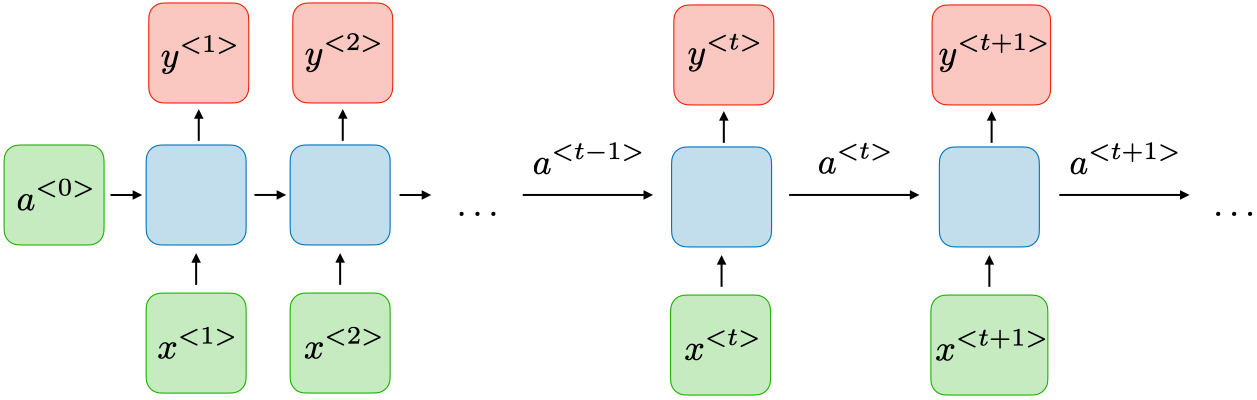
\includegraphics[width=0.8\textwidth]{asset/a_rnn.png}
  \caption{传统RNN网络结构}
  \label{rnn}
\end{figure}

\subsection{LSTM}
LSTM\ref{lstm}是一种特殊类型的RNN,它在一定程度上解决了RNN会梯度消失的问题,还能提供对长期记忆的理解和表达。
LSTM的关键通过被称为遗忘门、输入门和输出门的三个门来控制信息上下文在神经元之间的流动。
遗忘门决定了应该保留多少长期记忆,可以使用sigmoid函数来控制信息的保留。通过sigmoid函数将输入映射到在0和1之间变化的输出,0即不保留任何信息,1则保留单元状态的所有信息。
输入门决定将哪些信息添加到单元状态,从而添加到长期记忆中;输出门决定单元状态的哪些部分构建输出,从这个角度来讲,输出门负责短期记忆。总的来说,状态通过遗忘门和输入门更新。

LSTM的关键是单元状态,在单元的输入传递到输出的过程中,单元状态允许信息沿着整个链流动,仅通过三个门进行较小的线性动作。
通过三个门控,以过滤器的方式控制信息流并确定保留或忽略哪些信息。
LSTM的主要优点是它可以同时捕获序列的长期和短期模式,但由于结构更复杂,LSTM的计算成本更高,也就意味着训练时间更长。
\begin{figure}[htb]
  \centering
  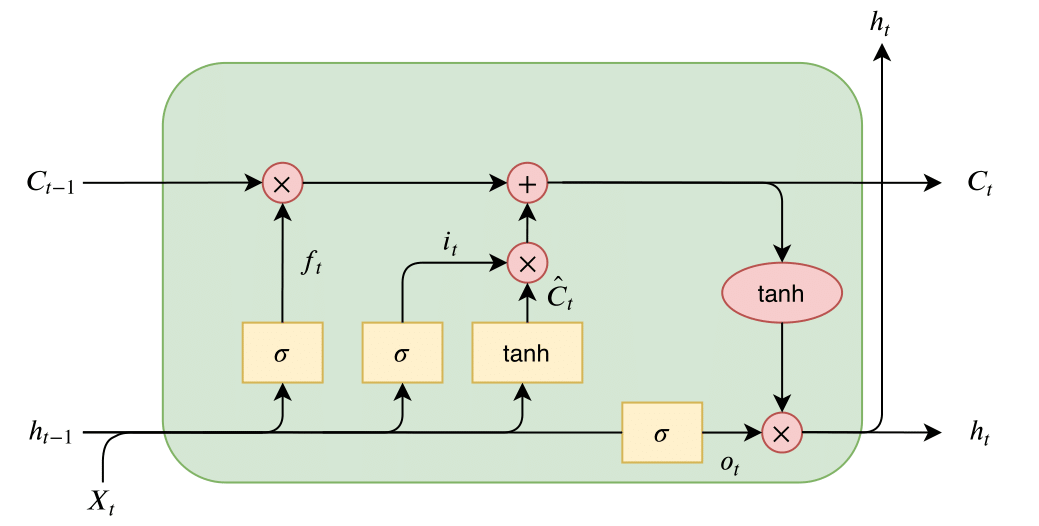
\includegraphics[width=0.8\textwidth]{asset/a_lstm.png}
  \caption{LSTM网络结构}
  \label{lstm}
\end{figure}

\subsection{GRU}
与LSTM类似,GRU\ref{gru}同样可以解决传统RNN的梯度消失问题。然而,与LSTM的不同之处在于GRU使用较少的门并且没有单独的内部存储器,或者说单元状态。
从这个角度来讲,GRU完全依赖隐藏状态作为记忆,这意味着GRU有着比LSTM更简单的架构。
GRU内部使用重置门和更新门来分别对长短期信息进行控制。重置门负责短期记忆,它决定保留和忽略多少过去的信息;更新门负责长期记忆,类似于LSTM的遗忘门。

当某一时间步需要更新隐藏状态时,他通过下述两个步骤来实现:
首先,确定所选择的隐藏状态,即当前输入和前一时间步的隐藏状态以及激活函数的组合。前一个隐藏状态对当前所选择的隐藏状态的影响由重置门控制;
然后,将所选择隐藏状态与上一时间步的隐藏状态相结合,生成当前隐藏状态。先前的隐藏状态和所选择隐藏状态如何组合由更新门决定。
如果更新门给出的值为0,则完全忽略先前的隐藏状态,这种情况下当前隐藏状态就是所选择的隐藏状态。如果更新门给出的值为1,需要做出的处理则完全相反。
由于与LSTM相比有着更简单的架构,GRU的计算效率更高,训练速度更快,需要更少的内存。
虽然GRU对过去的观察结果的考虑无法达到LSTM的程度,但是其已被证明对于较小的序列更有效。
\begin{figure}[htb]
  \centering
  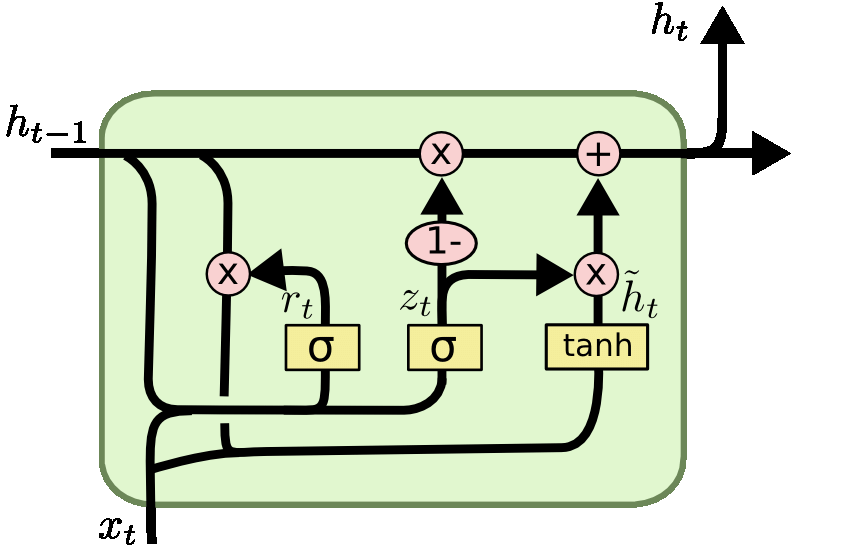
\includegraphics[width=0.8\textwidth]{asset/a_gru.png}
  \caption{GRU网络结构}
  \label{gru}
\end{figure}

\subsection{Transformer}
与RNN不同,Transformer\ref{transformer}则采用了一种完全不同的范式解决问题。
Transformer是一种基于注意力机制的序列到序列模型,其主要优点是能够并行处理输入序列,而不是像RNN那样顺序处理。这使得Transformer比RNN更快,更容易训练。
Transformer中没有了序列这个概念,通过将输入的语句当作一个整体传入embedding层中,赋予模型并行计算的能力,因为不再强调输入序列次序,也就没有长依赖的问题。
既然Transformer中不再使用循环结构,因此必须以不同的方式添加位置信息。
为了能够捕获序列中的位置信息,Transformer引入了\texttt{positional\_encoding}即位置编码的概念,
位置编码是一种向输入嵌入中添加位置信息的技术,它使模型能够理解输入中某些部分在整个输入中的位置。
这种方式在解决了序列顺序依赖的同时,也能将位置信息纳入模型考虑。
此外,Transformer还引入了自注意力机制作为核心组件。
与之前的机制不同的是,自注意力机制可以将序列中不同位置之间的依赖关系进行建模,不需要依赖于时间的顺序,因此可以更好地处理长序列。
\begin{figure}[htb]
  \centering
  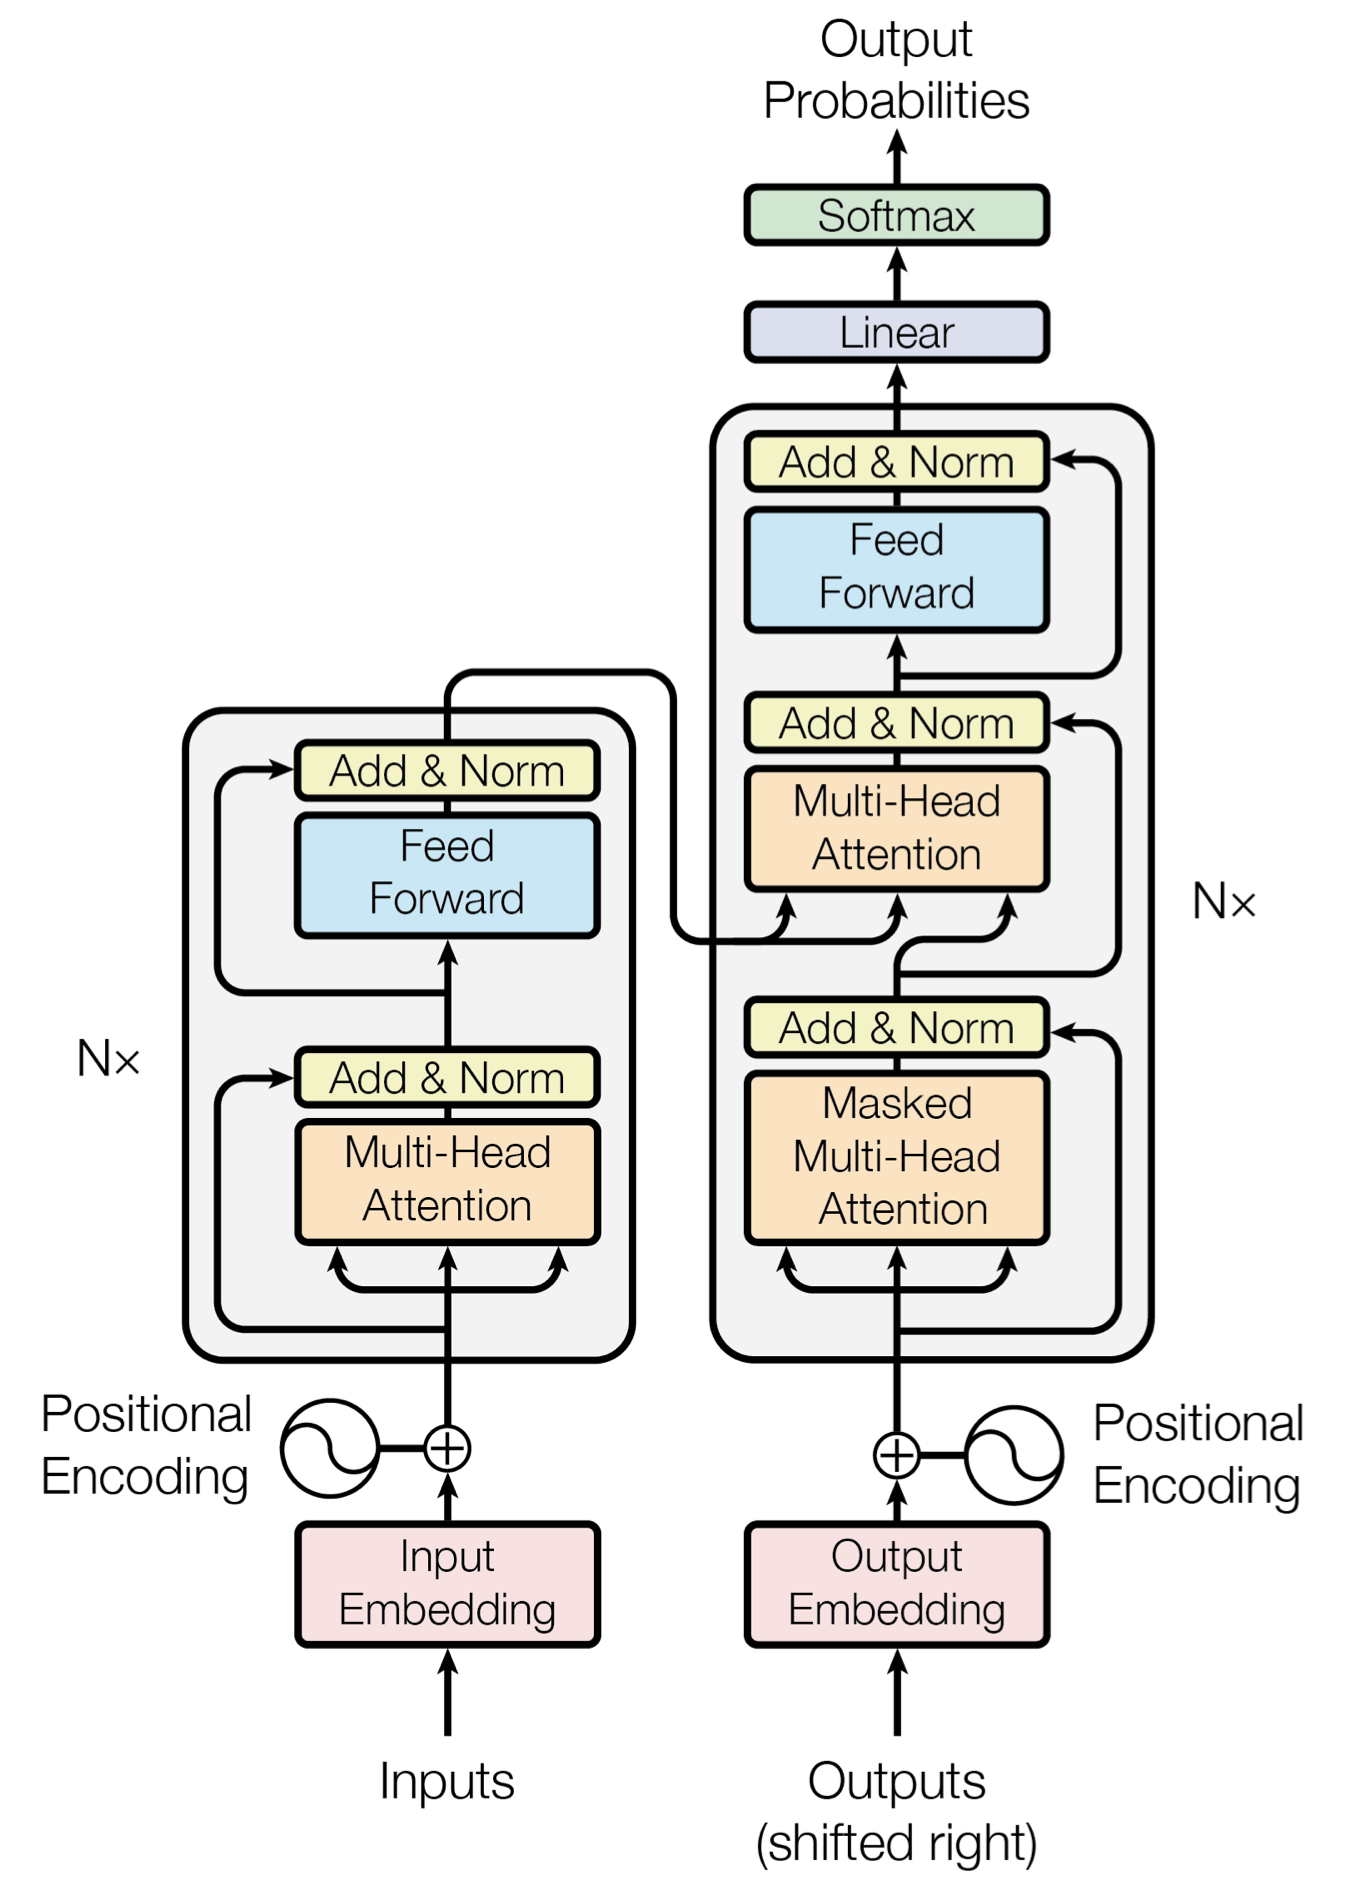
\includegraphics[width=0.5\textwidth]{asset/a_transformer.png}
  \caption{Transformer结构}
  \label{transformer}
\end{figure}

\newpage
\section{实验和超参数分析}
本部分将从模型选取和超参数设定两个角度对实验过程进行分析。
\subsection{同一参数下模型性能对比}
由于本实验中我们使用了多种不同的语言模型,为了能够对比其性能的差异,应保持参数的一致性,这里列举了两种不同参数配置下的实验结果。
\begin{table}[H]
  \centering
  \begin{tabular}{|c|c|c|c|c|c|c|c|c|c|c|c|c|}
    \hline
      \diagbox{评估指标}{模型选取}
      &RNN(Relu)&RNN(Tanh)&LSTM&GRU&Transformer\\
      \hline
      Test Loss&NA&5.26&\textbf{4.95}&5.26&6.55\\
      \hline
      Perplexity&NA&192.27&\textbf{141.38}&192.27&700.61\\
      \hline
  \end{tabular}
  \caption{Results with embedding size 200, hidden dimension 200}
  \label{tab1}
\end{table}

\begin{table}[H]
  \centering
  \begin{tabular}{|c|c|c|c|c|c|c|c|c|c|c|c|c|}
    \hline
      \diagbox{评估指标}{模型选取}
      &RNN(Relu)&RNN(Tanh)&LSTM&GRU&Transformer\\
      \hline
      Test Loss&NA&4.95&\textbf{4.90}&4.95&6.54\\
      \hline
      Perplexity&NA&141.47&\textbf{133.81}&141.47&694.68\\
      \hline
  \end{tabular}
  \caption{Results with embedding size 400, hidden dimension 200}
  \label{tab2}
\end{table}

可以看到,在本次实验的数据集和配置环境下,LSTM网络取得了最好的结果。
虽然Transformer在大规模数据集和大多数自然语言处理的任务场景下优秀的性能已经得到了验证,
但是当序列长度没有超过RNN的处理能力的时候,\texttt{positional\_encoding}对时序的建模能力还是不如RNN的。
我们本次实验所使用\texttt{gigaspeech}数据集规模并不大,可能无法很好地发挥Transformer模型的优势。

\subsection{不同超参数对模型性能的影响}
在本次实验中,我取得的最优性能是在使用LSTM模型下得到的,即表格\ref{tab2}中在测试集上的test loss 4.90和perplexity 133.81。
具体使用的参数配置为:
embedding size: 400,
hidden dimension: 200,
number of layers: 2,
initial learning rate: 20,
bptt: 35,
dropout rate: 0.2,
batch\_size: 20,
clip: 0.25,
epochs: 40,
Vocabulary Size: 27710,
Total number of model parameters: 17.46M.

从语义信息的角度来讲,提高embedding size和hidden dimension的大小,都能够更好地表征确定数据集下的语义信息,
即通过提升模型的参数量来提供更多的表征。在一定范围内,实验结果也确实表明更高的维度能够带来低的perplexity。
但是embedding size和hidden dimension也不是越大越好,过大的情况下,不但由于模型参数量的提升带来过多的训练开销,
还会因为模型的参数规模并不能很好地适配数据集规模而带来过拟合等问题,导致模型并不能很好地学到属于特定数据集的特征。

在本次实验过程中,由于适配了动态学习率调整的方法,在训练的过程中会根据参数更新的情况动态减小学习率,
所以初始learning rate并不会对最终模型的性能产生较大的影响。在模型训练的开始,可以使用比较大的学习率,帮助模型更快地参数更新。
为了适当地减少过拟合的问题,设定了drop out几率,一定的drop out rate可以使神经元随机失活,从而减少过拟合,但是drop out rate也不能过高,需要根据经验和实际的使用场景进行设置。

\section{Tensorboard支持}
为更好地观察和对比不同模型在统一参数下的运行结果,可以使用Tensorboard对training和validation过程中的loss进行绘图。
使用Tensorboard不但能够画出训练、验证和测试过程中的loss趋势等信息,还能够提供实时观看的功能,而不必等到训练全部完成之后再整体查看训练图,
从而能更早发现和定位训练过程出现的bug。
在使用服务器的情况下,由tensorboard的\texttt{Summary Writer}类记录结果,通过调用\texttt{tensorboard --logdir}命令
并指定端口接收远端服务器传回的消息,并在localhost进行查看,所得到的训练图像见附录部分\ref{tensor1}\ref{tensor2}。



\newpage
\section*{附录:Tensorboard训练图}
\begin{figure}[htbp]
  \centering
  \subfigure[RNN\_Tanh训练曲线]{
  \label{dim1start}
  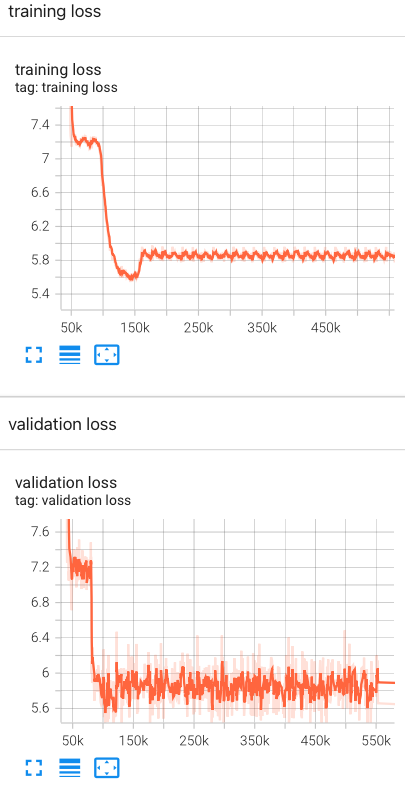
\includegraphics[width=0.45\textwidth]{asset/rnn_tanh.png}}
  \subfigure[LSTM训练曲线]{
  \label{dim1end}
  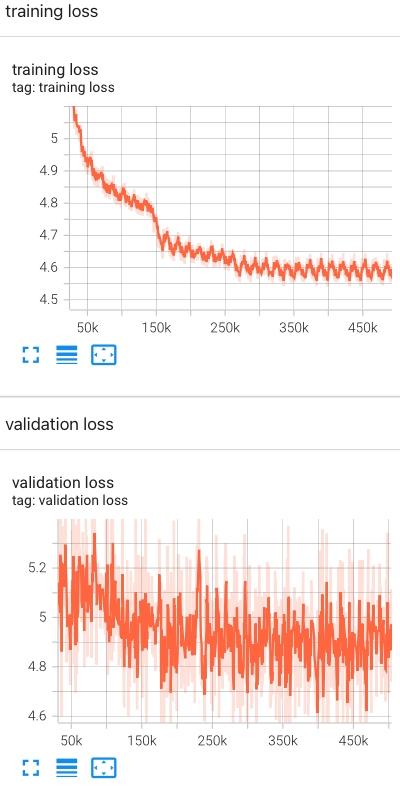
\includegraphics[width=0.45\textwidth]{asset/lstm.png}}
  \caption{Tensorboard结果展示}
  \label{tensor1}
\end{figure}

\begin{figure}[htbp]
  \centering
  \subfigure[GRU训练曲线]{
  \label{dim2start}
  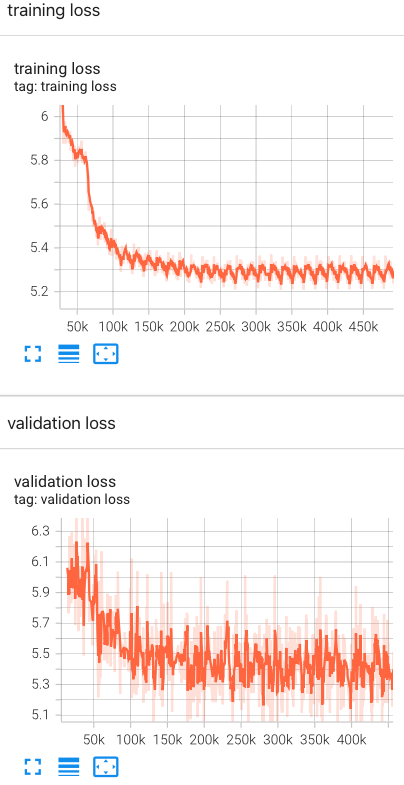
\includegraphics[width=0.45\textwidth]{asset/gru.png}}
  \subfigure[Transformer训练曲线]{
  \label{dim2end}
  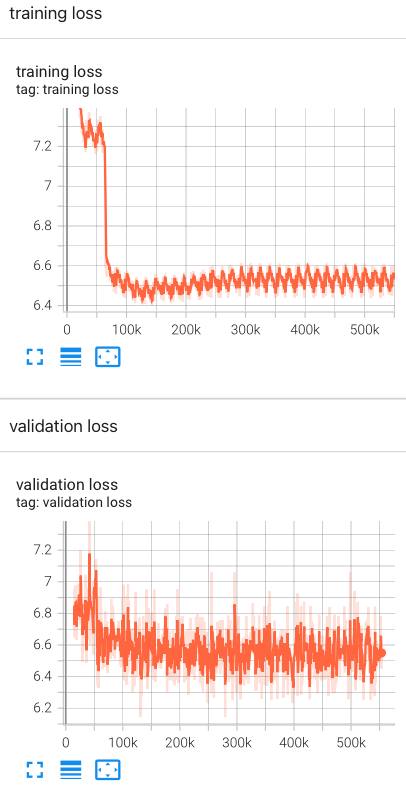
\includegraphics[width=0.45\textwidth]{asset/transformer.png}}
  \caption{Tensorboard结果展示}
  \label{tensor2}
\end{figure}

\end{document}

% below is table template used in Deep Learning courses
% \newpage
% \section{总结与思考}

% \begin{table}[H]
%     \centering
%     \begin{tabular}{|c|c|c|c|c|c|c|c|c|c|c|c|c|}
%       \hline
%         \diagbox{评估指标}{参数配置}
%         &\makecell{LR 1e-4\\WD 1e-4}
%         &\makecell{LR 3e-5\\WD 1e-4}
%         &\makecell{LR 5e-5\\WD 1e-4}
%         &\makecell{LR 7e-5\\WD 1e-4}
%         &\makecell{LR 1e-4\\WD 1e-4}
%         &\makecell{LR 1e-4\\WD 2e-4}\\
%         \hline
%         Pretrain&\Checkmark&\Checkmark&\Checkmark&\Checkmark&\XSolidBrush&\XSolidBrush\\
%         \hline
%         Best P.&.9188&.9172&\textbf{.9262}&.9228&.8250&.8393\\
%         \hline
%         Best R.&.9188&.9172&\textbf{.9262}&.9228&.8250&.8393\\
%         \hline
%         Best F1.&.9188&.9172&\textbf{.9262}&.9228&.8250&.8393\\
%         \hline
%         Final P.&.8046&\textbf{.9128}&.8873&.8711&.8003&.7816\\
%         \hline
%         Final R.&.8046&\textbf{.9128}&.8873&.8711&.8003&.7816\\
%         \hline
%         Final F1.&.8046&\textbf{.9128}&.8873&.8711&.8003&.7816\\
%         \hline
%         \diagbox{评估指标}{参数配置}
%         &\makecell{LR 1e-4\\WD 3e-4}
%         &\makecell{LR 1e-4\\WD 7e-5}
%         &\makecell{LR 1e-4\\WD 8e-5}
%         &\makecell{LR 3e-5\\WD 1e-4}
%         &\makecell{LR 5e-5\\WD 1e-4}
%         &\makecell{LR 7e-5\\WD 1e-4}\\
%         \hline
%         Pretrain&\XSolidBrush&\XSolidBrush&\XSolidBrush&\XSolidBrush&\XSolidBrush&\XSolidBrush\\
%         \hline
%         Best P.&.8192&.8170&.8377&.8157&.8335&\textbf{.8426}\\
%         \hline
%         Best R.&.8192&.8170&.8377&.8157&.8335&\textbf{.8426}\\
%         \hline
%         Best F1.&.8192&.8170&.8377&.8157&.8335&\textbf{.8426}\\
%         \hline
%         Final P.&.7965&.8170&\textbf{.8268}&.8073&.7493&.8082\\
%         \hline
%         Final R.&.7965&.8170&\textbf{.8268}&.8073&.7493&.8082\\
%         \hline
%         Final F1.&.7965&.8170&\textbf{.8268}&.8073&.7493&.8082\\
%         \hline
%     \end{tabular}
%     \caption{不同参数配置下的运行结果}
%     \label{fig1}
% \end{table}